\section{Software}
\label{Sec:software}
\paragraph{
Coletado os dados, resta mostrar informações úteis ao usuário. Com o consumo de corrente e a voltagem da tomada, é possível calcular a potência e alguns outros dados interessantes para o usuário. O aplicativo desenvolvido nesse trabalho será responsável por esse tratamento e a visualização dos dados coletados pelos sensores. As funções principais são as seguintes:
}
\begin{itemize}
\item{realizar login}
\item{criar planos de consumo mensal máximo}
\item{visualizar o consumo através de gráficos por equipamento ou total}
\item{calcular o custo do consumo dos equipamentos por período}
\item{exportar os dados de consumo de um equipamento (ou mais)}
\item{importar os dados de consumo de um equipamento (ou mais)}
\end{itemize}
\subsection{Classes e atributos}
\textbf{Classe}: Equipment\\
\textbf{Descrição}: um equipamento monitorado\\	
\textbf{Atributos:}
\begin{enumerate}
  \item id (integer): Identificador do equipamento
  \item name (String): Nome do equipamento
  \item description (Text): descrição do equipamento 
  \item nominal\_power (float): potência do equipamento descrita no manual do equipamento 
  \item measurement\_unit (String): unidade do valor dado em nominal\_power
  \item approximated\_consumption (float): consumo aproximado do equipamento dado pelo fabricante 
\end{enumerate}

\textbf{Classe}: Sensor\\
\textbf{Descrição}: um sensor do sistema\\	
\textbf{Atributos:}
\begin{enumerate}
	\item id (integer): identificador do sensor dentro do software.
	\item name (String): nome dado pelo usuário para o sensor
	\item code (String): identificador do sensor entre outros sensores. Informação configurada no próprio módulo do sensor.
	\item equipment\_id (integer): equipamento a qual está associado
\end{enumerate}

\textbf{Classe}: Consumption\\
\textbf{Descrição}: Representa uma medida feita de um equipamento em um dado instante\\	
\textbf{Atributos:}
\begin{enumerate}
	\item id (integer): identificador do consumo
	\item moment (DateTime): a data e a hora de quando foi feita a medida
	\item current (float): corrente no momento da medida em amperes
	\item voltage (float): voltagem do tomada do equipamento. 220V ou 110V
\end{enumerate}

\subsection{Classes e atributos}
	\textbf{Classe}: User\\
	\textbf{Descrição}: Representa um usuário do sistema\\	
	\textbf{Atributos:}
\begin{enumerate}
	\item id (integer): identificador do usuário
	\item name (String):  Nome do usuário
	\item username (String): Nome de usuário usado para efetuar o login
	\item password (String com Criptografia): Senha do usuário usada para efetuar o login
    \item income\_type (String): O tipo de renda do usuário, Residencial ou Residencial de baixa renda, definida pela AES eletropaulo.
\end{enumerate}

\subsection{Classes e atributos}
	\textbf{Classe}: Goal\\
	\textbf{Descrição}: Representa uma meta de consumo por mês.\\
	\textbf{Atributos:}
\begin{enumerate}
	\item id (integer): identificador da meta
	\item name (String):  Nome da meta
	\item value\_in\_percent (float): Consumo pretendido em percentagem (em relação ao mês anterior)
	\item yearmonth\_start (DateTime): Mês/Ano de início do período da meta
    \item yearmonth\_end (DateTime): Mês/Ano de fim do período da meta
\end{enumerate}

\subsection{Classes e atributos}
	\textbf{Classe}: AESRate\\
	\textbf{Descrição}: Representa a taxa de conversão da AES eletropaulo de kilowatts hora para reais. Esses valores são obtidos através do site da AES Eletropaulo: \url{https://www.aeseletropaulo.com.br/poder-publico/prazos-e-tarifas/conteudo/tarifa-de-energia-eletrica}\\
	\textbf{Atributos:}
\begin{enumerate}
	\item id (integer): identificador da taxa de conversão
	\item value (float): O valor da taxa de conversão no instante
	\item date (DateTime): O instante que a taxa de conversão foi buscada
	\item range\_start (float): O início da faixa que define a taxa de conversão
    \item range\_end (float): O início da faixa que define a taxa de conversão
\end{enumerate}

\paragraph{No sistema é possível cadastrar apenas uma entidade principai os equipamentos eletrônicos monitorados, sendo prevista a possibilidade de que um sensor possa mudar de um equipamento para outro, sendo que tal mudança deve ser cadastrada no sistema pelo  usuário na tela de configurações, como mostrado na tela de configurações no diagrama de navegação.  Essa possibilidade de mudança da configuração dos sensores explica a relação do equipamento e as medidas de consumo: caso o usuário troque o sensor de equipamento ainda será possível visualizar dados anteriores de outros equipamentos já monitorados.
Os sensores devem ser criados automaticamente pelo sistema uma vez que eles sejam colocados no sistema. Eles enviam um sinal inicial que informa seu identificador para que o sistema o cadastre. O usuário poderá, então, colocar um nome que preferir nesse sensor.\\
Adquiridas as medidas, é possível vizualizar esses dados em uma tabela de consumo na tela de consumo. Nessa tela, é possível construir o gráfico do consumo em função de vários períodos de tempo, no caso, o consumo por dia e por mês, assim como metas de consumo de energia dos equipamentos selecionados e previsões de consumo que serão calculadas a partir do consumo nominal dos equipamentos.
}

\begin{figure}[H]
\begin{center}
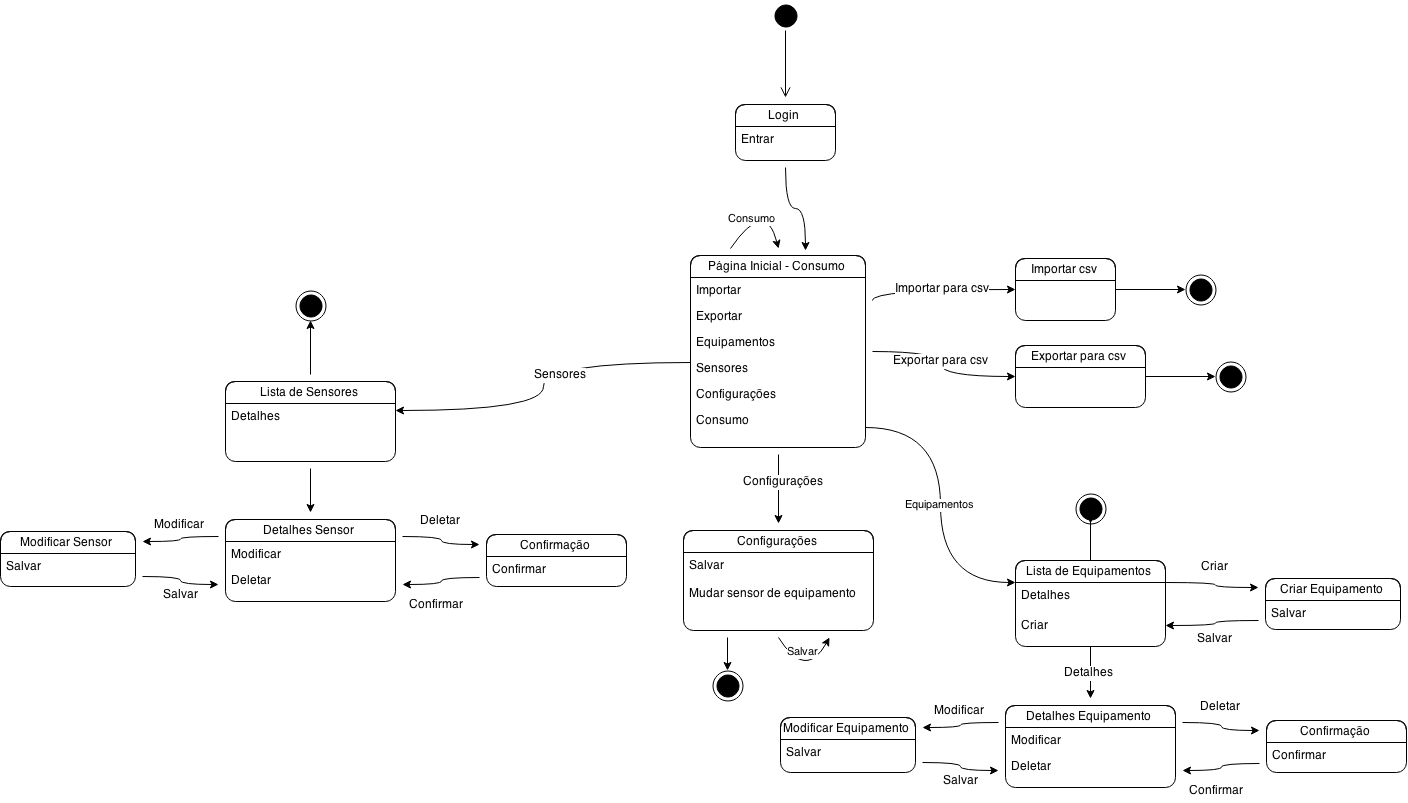
\includegraphics[width=10cm,height=10cm,keepaspectratio]{figuras/diagrama_navegacao.png}
\caption{\label{fig:diagrama navegacao} Diagrama de Navegação}
\end{center}
\end{figure}

\begin{figure}[H]
\begin{center}
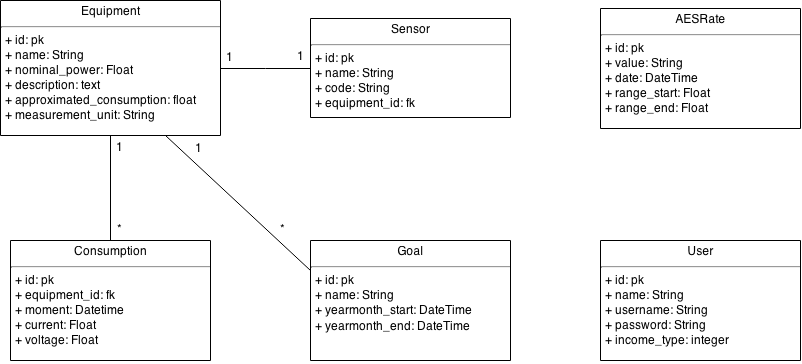
\includegraphics[width=10cm,height=10cm,keepaspectratio]{figuras/diagrama_classes.png}
\caption{\label{fig:diagrama classes} Diagrama de Classes}
\end{center}
\end{figure}

\subsection{Regras de negócio}
\paragraph{As medidas serão feitos em uma taxa de uma vez a cada dez minutos, o que leva a 6 amostras por hora, 144 por dia e 4320 por mês. Dado que cada amostra é uma linha de uma tabela, torna-se necessário algum tipo de redução desses dados para que o banco na nuvem não chegue a seu ponto máximo, dado que no projeto será usado um serviço cloud com taxa gratuita e, portanto, muito limitada. Logo, foi decidido que a janela temporal que o usuário conseguirá visualizar será restrita ao mês anterior e o mês atual quando o gráfico for uma função das horas do dia, e os outros dados mais antigos serão agrupados em meses para que ainda possa ser possível visualiza-los quando o gráfico for uma função dos meses. Caso seja necessário, será usado um plano pago, o que resolveria esse problema.
}

\subsection{Tecnologia}
\paragraph{Para o aplicativo será utilizado o framework Django, devido ao uso da linguagem python, que é uma linguagem limpa, de fácil utilização e com ampla disponibilidade de bibliotecas gratuitas e de fóruns para auxílio na implementação.
Há também algumas outras razões para escolher tais ferramentas:
Uma das vantagens do python nesse caso é uma pequena vantagem de compatibilidade, uma vez que o \"pi\" em \"raspberry pi\" vem de \"python\", já que o hardware foi construído com a intenção do aprendizado de programação com python (apesar da possibilidade de usar outras linguagens). Outra vantagem provinha do conhecimento prévio dos integrantes do grupo e do framework que reduzia muito o tempo de desenvolvimento. E por último, a possibilidade de, se necessário, rodar o servidor da aplicação no próprio raspberry sem a necessidade de acrescentar muitos outros módulos externos, uma vez que no raspberry python já é uma linguagem nativa, sendo necessário instalar apenas as dependências do django.
}